\section{Admin Module: Complaint Resolution System}
To address student grievances, the Admin panel provides a real-time tracking system for complaints submitted through the student portal.

\subsection{Reviewing Pending Complaints}
All student issues are listed in a simplified queue, allowing administrators to address them systematically.

\begin{figure}[H]
    \centering
    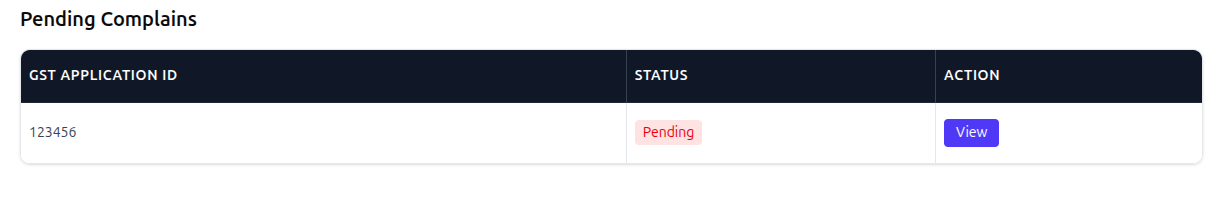
\includegraphics[width=0.85\textwidth]{chapters/chapter4/images/checkcomplain.png}
    \caption{Pending Complaint Tracking Interface}
    \label{fig:check_complain}
\end{figure}

The complaint handling workflow involves:
\begin{itemize}
    \item \textbf{Application ID Mapping:} Every complaint is mapped to a GST Application ID for cross-verifying academic records.
    \item \textbf{Detailed Action:} By clicking the "View" button, the admin can read the full text of the complaint and take necessary corrective measures.
\end{itemize}